\documentclass[a4paper]{report}

\usepackage{NielsPackage}

\lstset{language=HTML}

\hypersetup{
	pdfauthor = {Niels Doorn},
	pdftitle = {Javascript Introductie},
	pdfsubject = {HTML, CSS, JavaScript},
	pdfkeywords = {HTML,css,lesbrief},
	pdfcreator = {NielsDoorn/RocVanTwente}
}

\rhead{\textsc{Javascript Introductie}}
\lhead{}
\chead{}
\lfoot{Niels Doorn \copyright~2012}
\cfoot{}
\rfoot{\thepage}

\fancypagestyle{plain}{
	\fancyhf{}
	\fancyfoot[L]{Niels Doorn, ROC van Twente \copyright~2012}
	\fancyfoot[C]{}
	\fancyfoot[R]{\thepage}
	\renewcommand{\headrulewidth}{0pt}
	\renewcommand{\footrulewidth}{0.4pt}
}

\begin{document}

\chapter*{\textcolor{seccol}{Javascript} Introductie}

\section*{Inleiding}
\addcontentsline{toc}{section}{Inleiding}
JavaScript is een programmeertaal die je kunt gebruiken om interactie toe te voegen aan een website. JavaScript is onderdeel van de HTML5 standaard en biedt vele mogelijkheden om van een website een web applicatie te maken.

Deze lesbrief bevat een aantal opdrachten die je moet maken en in moet leveren. Ze worden beoordeelt door je docent en vormen een deel van je cijfer voor deze periode. Voor deze opdrachten heb je een les (twee keer drie kwartier) de tijd!

We beginnen met wat uitzoek vragen en daarna mag je echt aan het werk!

\section*{Op zoek naar JavaScript}
\addcontentsline{toc}{section}{Op zoek naar JavaScript}

\subsection*{Opdracht 1}
Zoek op internet uit welke onderdelen HTML5 bevat die gebruik maken van JavaScript. Het gaat dan om functies die voor HTML5 nog niet beschikbaar waren.

\subsection*{Opdracht 2}
Ga op zoek naar een website die gebruik maakt van een of meerdere van deze nieuwe mogelijkheden van HTML5. Geef de URL van de website.

\subsection*{Opdracht 3}
Noem drie dingen waar je javascript voor zou willen gebruiken in een website.

\section*{JavaScript gebruiken}
\addcontentsline{toc}{section}{JavaScript gebruiken}
JavaScript heeft alleen een browser nodig om te werken. Echter, het is net als bij andere programmeertalen handig om wat tools te gebruiken om je te helpen met programmeren.

De meeste browser hebben tegenwoordig mogelijkheden om als ontwikkelaar te zien wat er goed of fout gaat in de browser. Zo kun je bij Chrome de ontwikkelaars modus aanzetten bij instellingen en kun je bij Firefox de plugin Firebug installeren. 

Daarnaast kun je Dreamweaver of een andere editor gebruiken om JavaScript te schrijven.

\subsection*{Hello World!}
Het is een beetje obligaat, maar laten we toch maar beginnen met een Hello World programma in JavaScript! Wat hebben we nodig, een HTML pagina en een JavaScript pagina. De JavaScript pagina moeten we koppelen aan de HTML pagina. Hieronder zie je dat je dat met de \emph{script} tag kunt doen.

\lstinputlisting{code/helloworld.html}

\noindent De bijbehorden JavaScript file bevat slechts een regel code die in het `console' hello world laat zien.

\lstinputlisting{code/helloworld.js}

\noindent Je kunt met behulp van Firebug of de ontwikkelaarstools van Chrome het console laten zien, hieronder zie je een screenshot van Chrome.

\begin{center}
\resizebox{110mm}{!}{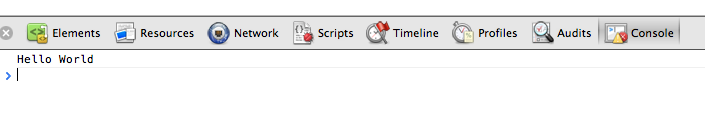
\includegraphics{console}}
\end{center}

\noindent \textbf{Opdracht:} Maak een HTML file, een JavaScript file en koppel deze. Zorg ervoor dat je firebug o.i.d. geinstalleerd hebt en toon het console met Hello World. Laat je docent dit zien!

\subsection*{Genoeg van Hello World? Laten we iets leuks gaan doen!}
Vanuit JavaScript kunnen we de DOM van je HTML veranderen. Dit is een van de sterke kanten van JavaScript. Neem het voorbeeld hieronder over en kijk wat er gebeurd als je op het blokje klikt.

\noindent HTML:
\lstinputlisting{code/intro.html}

\noindent CSS:
\lstinputlisting{code/style.css}

\noindent JavaScript:
\lstinputlisting{code/script.js}

\noindent \textbf{Opdracht 1:} Pas de JavaScript code zo aan dat het blokje 20px aan alle kanten groter wordt.
\\
\\
\noindent \textbf{Opdracht 2:} Pas de JavaScript code zo aan dat het blokje 45 graden roteerd.
\\
\\
\noindent \textbf{Opdracht 3:} Pas de JavaScript code zo aan dat het blokje weer wit wordt als je nogmaals klikt.
\\
\\
\noindent \textbf{Opdracht 4:} Pas de \textbf{CSS} code zo aan dat alle aanpassingen aan het blokje geleidelijk gaan (hint: transitions).

\end{document}